\input{../000_header_year.txt}

\begin{document}

%++++++++++++++++++++++++++++++++++++++++++++++++++++++++++++++++++++++++++++++++
%++++++++++++++++++++++++++++++++++++++++++++++++++++++++++++++++++++++++++++++++
%++++++++++++++++++++++++++++++++++++++++++++++++++++++++++++++++++++++++++++++++
\exheader
%++++++++++++++++++++++++++++++++++++++++++++++++++++++++++++++++++++++++++++++++
%++++++++++++++++++++++++++++++++++++++++++++++++++++++++++++++++++++++++++++++++
%++++++++++++++++++++++++++++++++++++++++++++++++++++++++++++++++++++++++++++++++


\noindent
{\bf 電気回路　$LCR$回路}　電気回路は$C$の電圧，$L$の電流を状態とすると状態方程式が求められる．以下の回路の状態方程式を求めよ．

\begin{minipage}{100mm}
　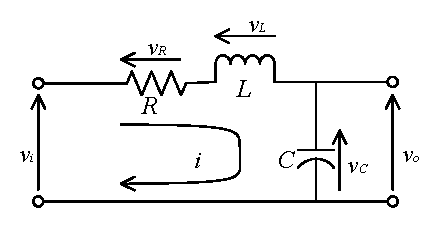
\epsfig{file=LCR.eps,scale=1.3}
\end{minipage}
\begin{minipage}{50mm}
回路の基本方程式
\begin{align*}
	v_L & = L \frac{d i}{dt} \\
	i & = C \frac{d v_C}{dt} \\
	v_R &= i R \\
	v_i & = v_L + v_C + v_R \\
	v_o & = v_C
\end{align*}
\end{minipage}

\vfill

\begin{tabular}{|l|}
\hline
解答：状態方程式\\[3cm]
\hspace*{15cm}\\
\hline
\end{tabular}


%---------------------------------------------------------------------------
\newpage

\noindent
{\bf 電気回路　$LCR$回路}　電気回路は$C$の電圧，$L$の電流を状態とすると状態方程式が求められる．以下の回路の状態方程式を求めよ．

\begin{minipage}{100mm}
　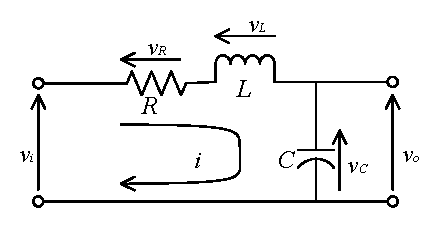
\epsfig{file=LCR.eps,scale=1.3}
\end{minipage}
\begin{minipage}{50mm}
回路の基本方程式
\begin{align*}
	v_L & = L \frac{d i}{dt} \\
	i & = C \frac{d v_C}{dt} \\
	v_R &= i R \\
	v_i & = v_L + v_C + v_R \\
	v_o & = v_C
\end{align*}
\end{minipage}
\ \\[1cm]

状態を$i$, $v_C$とするとその微分が必要だから
\begin{align*}
	\frac{d i}{dt} 
	&= \frac{v_L}{L} 
	= \frac{v_i - v_C - v_R}{L} 
	= - \frac{1}{L} v_R - \frac{1}{L} v_C + \frac{1}{L} v_i 
\\ &
	= - \frac{1}{L} R i - \frac{1}{L} v_C + \frac{1}{L} v_i 
	= - \frac{R}{L} i - \frac{1}{L} v_C + \frac{1}{L} v_i \\
	\frac{d v_C}{dt}
	&= \frac{i}{C} 
	= \frac{1}{C} i \\
	v_o &= v_C 
\end{align*}
よって状態方程式は
\begin{align*}
	\frac{d}{dt}
	\left (
	\begin{array}{c}
		i \\
		v_C
	\end{array}
	\right )
	&=
	\left (
	\begin{array}{cc}
		-\frac{R}{L} & -\frac{1}{L} \\
		\frac{1}{C} & 0 \\
	\end{array}
	\right )
	\left (
	\begin{array}{c}
		i \\
		v_C
	\end{array}
	\right )
	+
	\left (
	\begin{array}{c}
		\frac{1}{L} \\
		0
	\end{array}
	\right )
	v_i
\\
	v_o 
	&=
	\left (
	\begin{array}{cc}
		0 & 1 
	\end{array}
	\right )
	\left (
	\begin{array}{c}
		i \\
		v_C
	\end{array}
	\right )
\end{align*}


\end{document}

